
\section{IV - Problème de reproduction de l'opérateur XOR}
\begin{frame}{IV - Problème de reproduction de l'opérateur XOR}
	\begin{block}{Problème non linéairement séparable}
		Une couche de perceptron ne peut pas reproduire les opérateurs non linéairement séparables. \\
		Il faut mettre des couches de perceptron en série (couches cachées) pour pouvoir reproduire ces opérateurs. \\
	\end{block}
	\begin{figure}
		\centering
		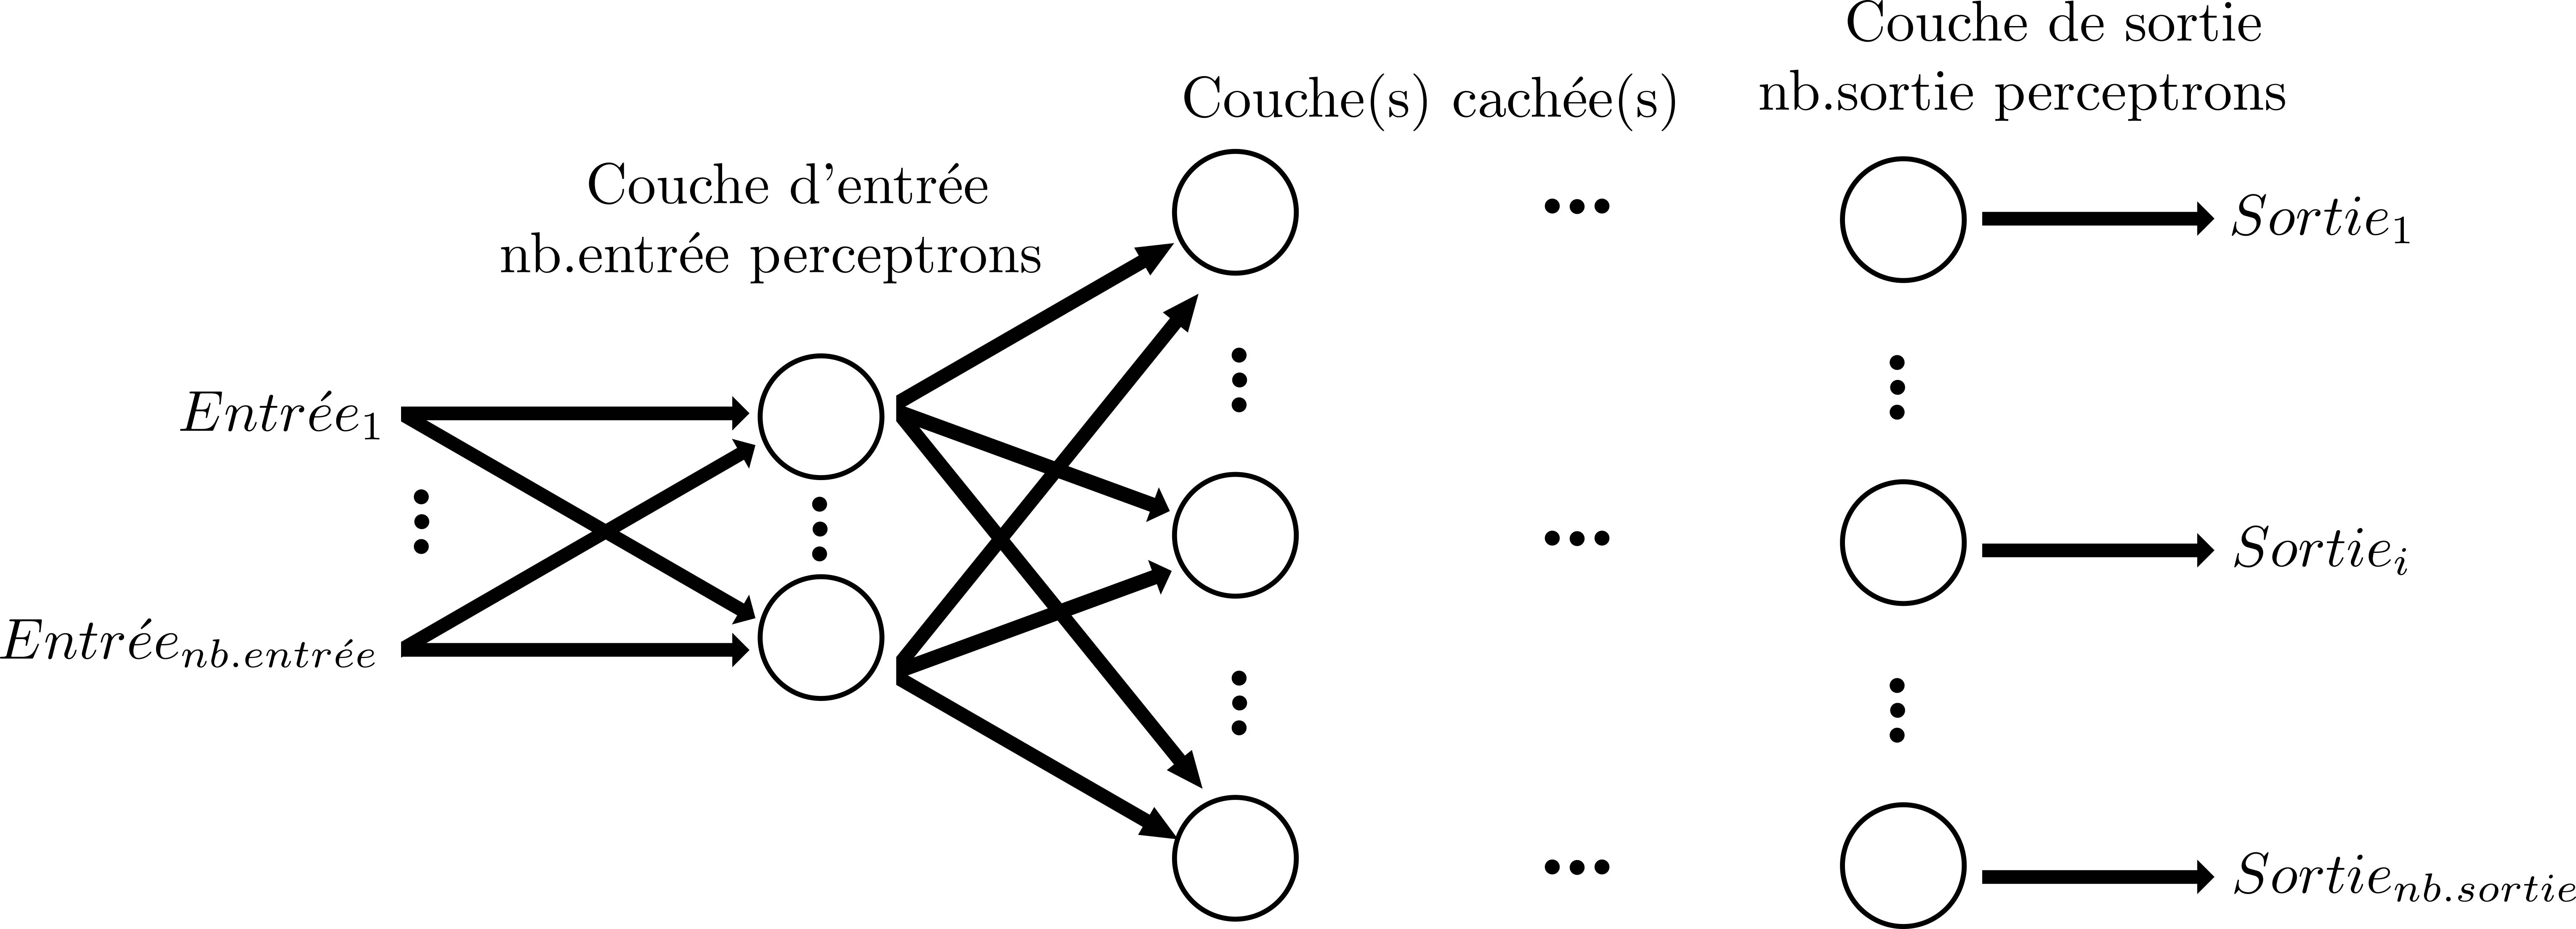
\includegraphics[height=120px]{1-Reseau.png}
		\caption{Schéma d'un réseau de neurones}
	\end{figure}
\end{frame}


\begin{frame}{IV - Problème de reproduction de l'opérateur XOR}
	\begin{block}{Le XOR nécessite un réseau}
		Le XOR, \og $ou\ exclusif$ \fg, est un opérateur non linéairement séparable. \\
	\end{block}
	\begin{figure}
		\centering
		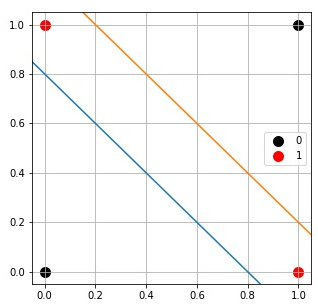
\includegraphics[width=150px]{2-XOR.jpg}
		\caption{Schéma de l'opérateur XOR}
	\end{figure}
\end{frame}


\begin{frame}{IV - Problème de reproduction de l'opérateur XOR}
	\begin{figure}
		\centering
		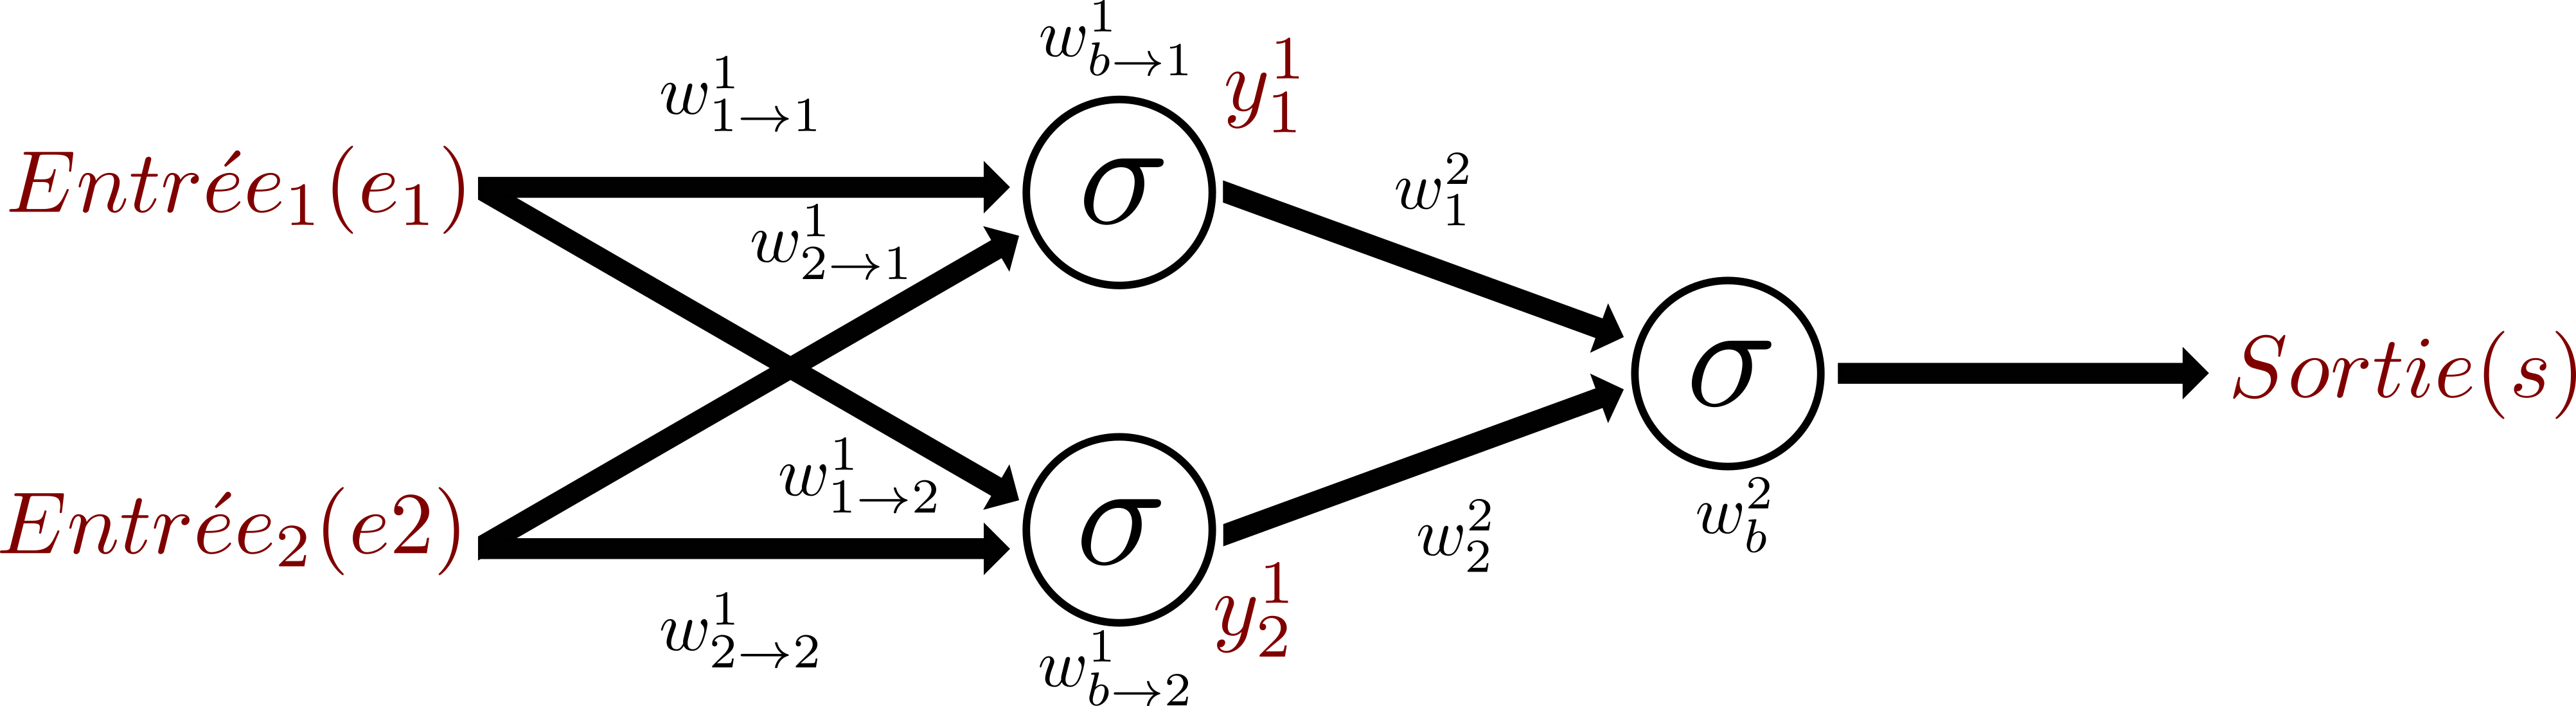
\includegraphics[width=\textwidth]{3-Model.png}
		\caption{Schéma du réseau de neurone reproduisant le XOR}
	\end{figure}
%	\begin{block}{Descente de gradient}
%		$w \leftarrow w - t \dfrac{\partial f}{\partial w}$ où $t$ est le taux d'apprentissage et $f$ la fonction de coût
%	\end{block}
%	\begin{exampleblock}{Exemple}
%		• $\dfrac{\partial f}{\partial w^2_1} = 2(s - s_{attendue})\sigma_2 'y^1_1$ \\
%		• $\dfrac{\partial f}{\partial w^1_{1\to 1}} = 2(s - s_{attendue})\sigma_2 'w^2_1 \sigma _{1} ' e_{1}$
%	\end{exampleblock}
\end{frame}


\begin{frame}{IV - Code}
	\lstinputlisting[language=Python, firstline=15]{1-XOR.py}
\end{frame}


\begin{frame}{IV - Apprentissage de la reproduction du XOR}
	\begin{figure}
		\centering
		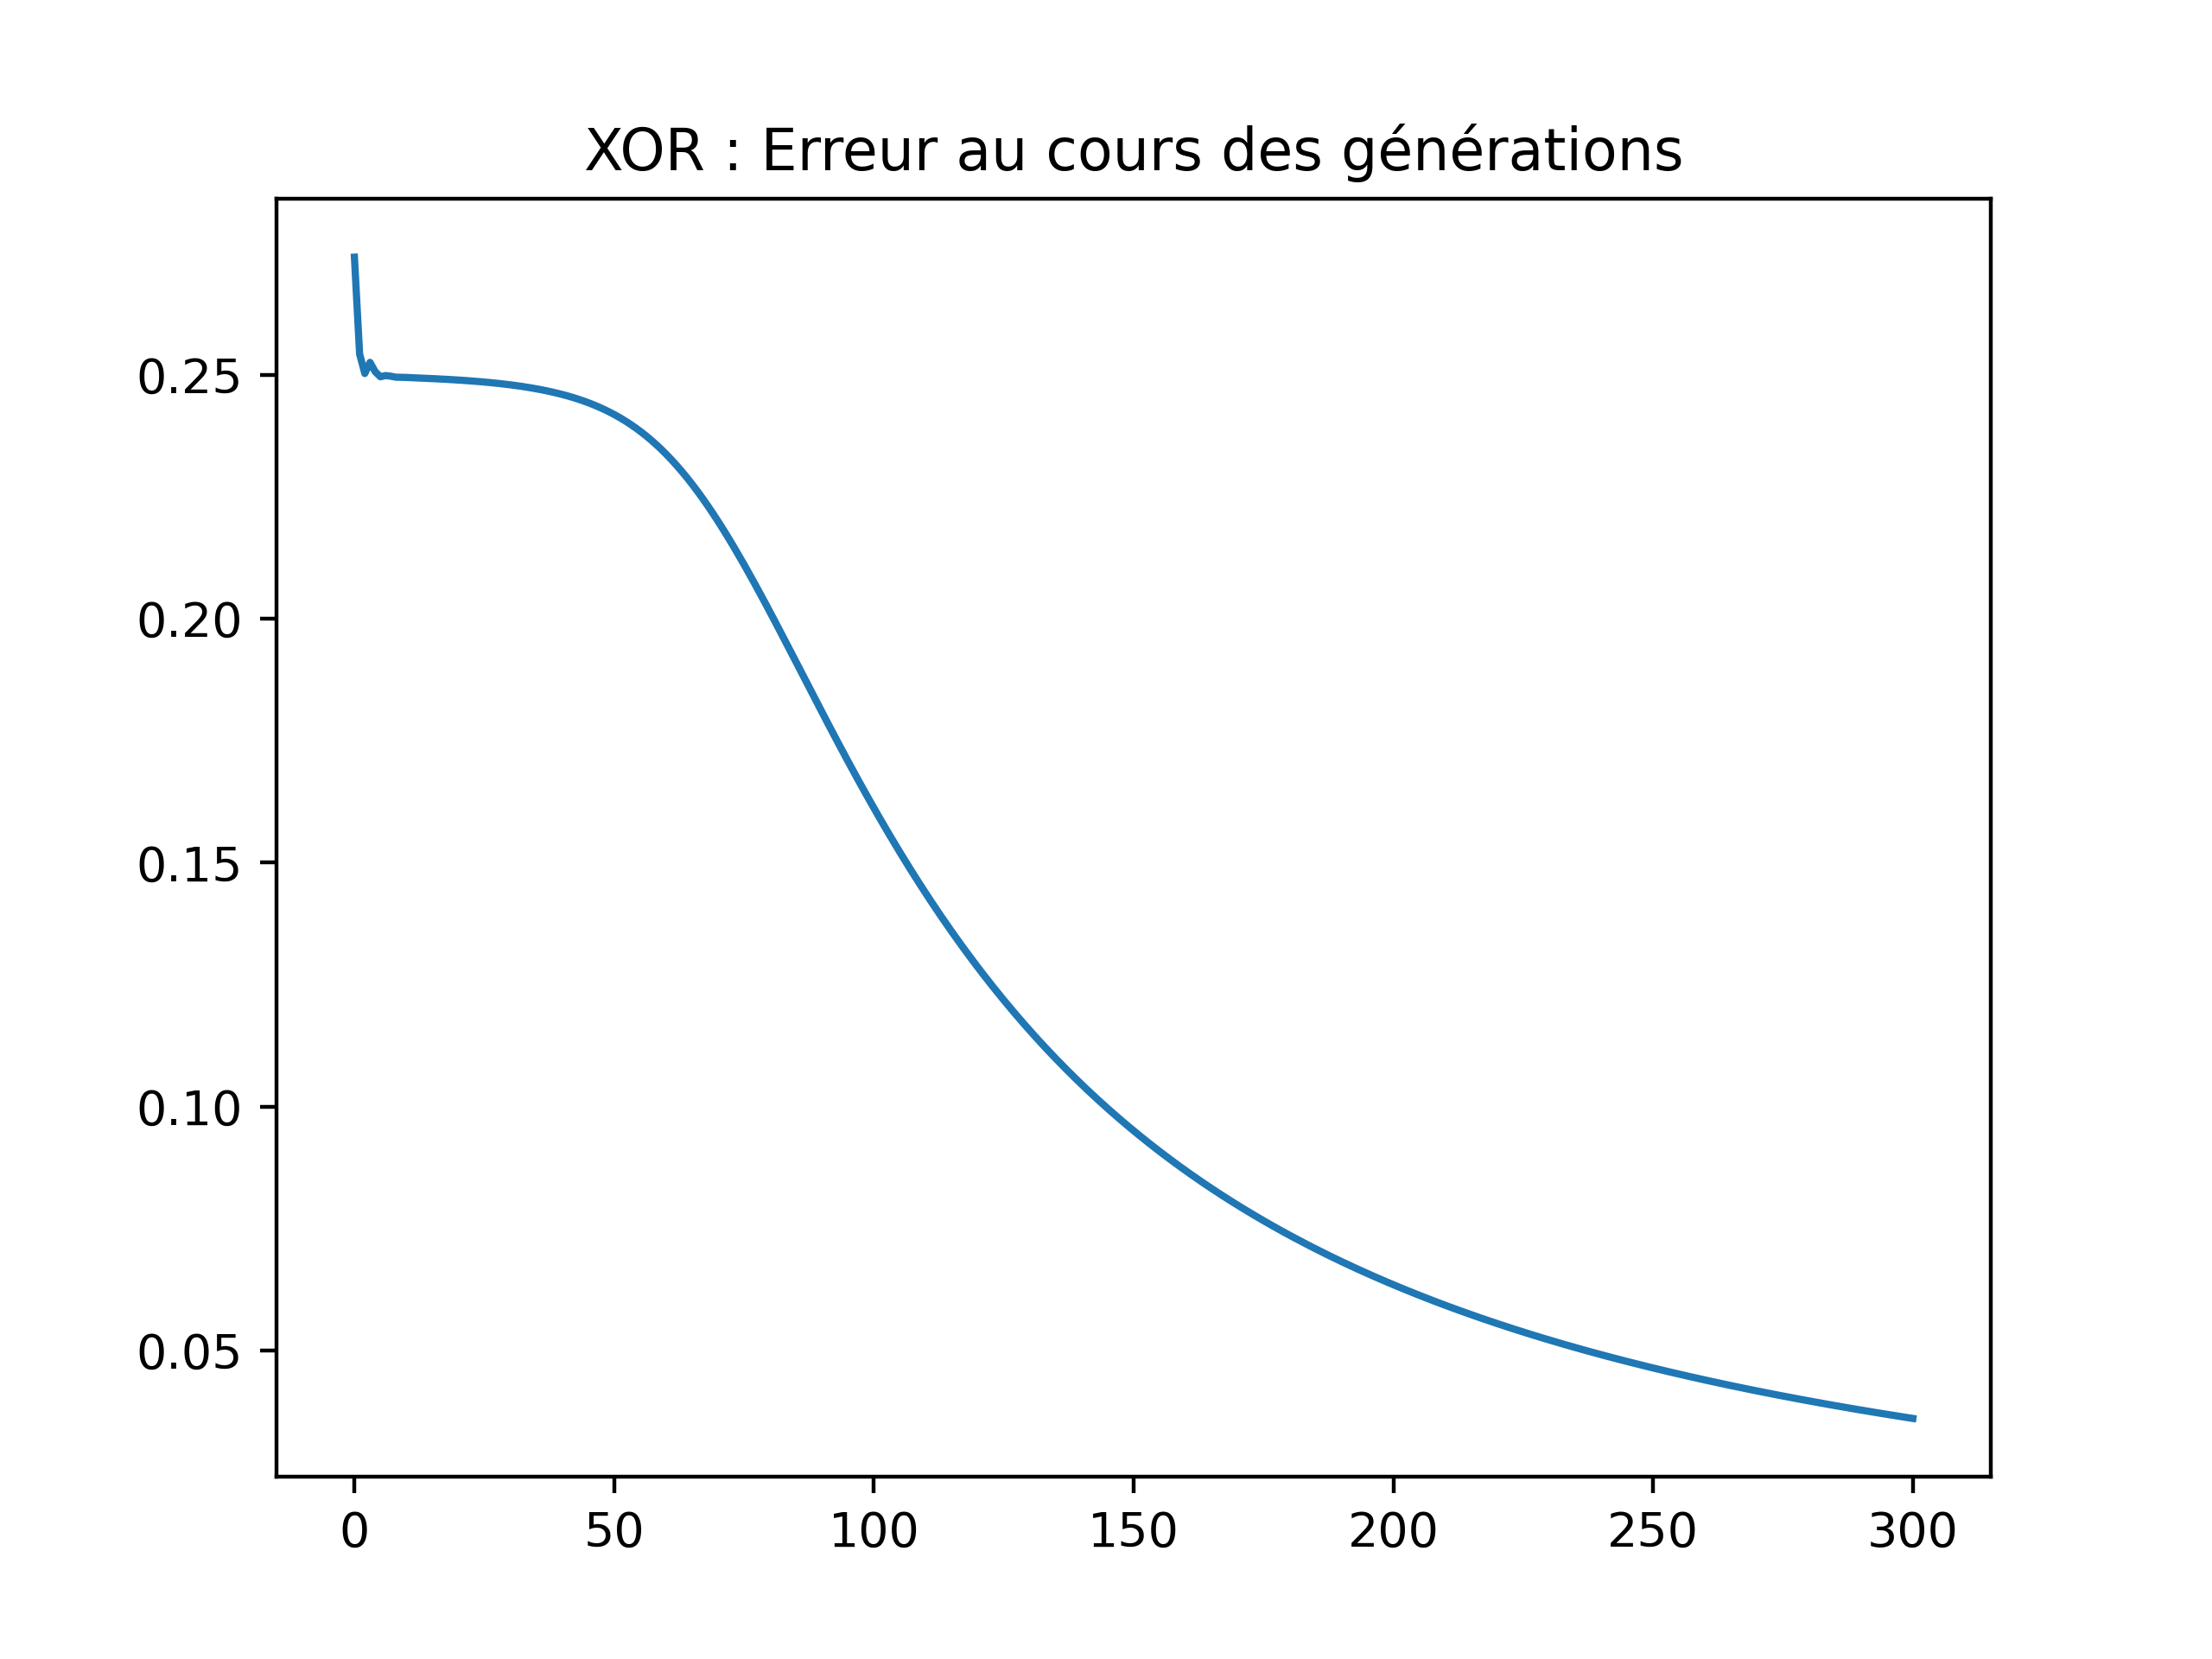
\includegraphics[width=270px]{4-XOR.png}
		\caption{Erreur sur la reproduction du XOR au cours de l'apprentissage}
	\end{figure}
\end{frame}


\begin{frame}{IV - Mes résultat}
	\begin{block}{Données}
		• 4 données \\
		• 300 générations \\
		• Erreur minimale atteinte 0.036
	\end{block}
	\begin{align*}
		Entr\acute{e} e\, :
		\begin{pmatrix}
			0 & 0 \\
			0 & 1 \\
			1 & 0 \\
			1 & 1
		\end{pmatrix}
		 & \to
		\mathlarger{\mathlarger{\sigma_{couche1}}}
		\left( \centerdot \times
		\begin{pmatrix}
				0.85 & 5.42 \\
				0.85 & 5.40 
			\end{pmatrix}
		\right) \\
		 & \to
		\mathlarger{\mathlarger{\sigma_{couche2}}}
		\left( \centerdot \times
		\begin{pmatrix}
				-18.39 \\
				14.42  
			\end{pmatrix}
		\right) \\
		 & \to
		Sortie\, :
		\begin{pmatrix}
			0.12 \\
			0.81 \\
			0.81 \\
			0.24
		\end{pmatrix}
		Sortie_{attendue}\, :
		\begin{pmatrix}
			0 \\
			1 \\
			1 \\
			0
		\end{pmatrix}
	\end{align*}
\end{frame}